% % % % % % % % % % % % % % % % % % % % % % % % % % % % % % % % % % % % % % % % % % % %
%                                                                                     %
% Short Sectioned Assignment LaTeX Template Version 1.0 (5/5/12)                      %
% This template has been downloaded from: http://www.LaTeXTemplates.com               %
%                                                                                     %
% Original author:  Frits Wenneker (http://www.howtotex.com)                          %
%                                                                                     %
% Modified by: Fco Javier Sueza Rodríguez (fcosueza@disroot.org)                      %
%                                                                                     %
% Changes:                                                                            %
%	    - Custom Chapters, Sections and Subsections (titlesec package)                %
%           - Document type scrbook (oneside)                                         %
%           - Use babel-lang-spanish package and marvosym                             %
%           - Use hyperref, enumitem, tcolorbox and glossaries packages               %
%           - Use Time New Roman (mathptmx), Helvetic and Courier fonts               %
%                                                                                     %
% License: CC BY-NC-SA 3.0 (http://creativecommons.org/licenses/by-nc-sa/3.0/)        %
%                                                                                     %
% % % % % % % % % % % % % % % % % % % % % % % % % % % % % % % % % % % % % % % % % % % %

%-----------------------------------------------%
%	              Packages                  %
%-----------------------------------------------%

\documentclass[paper=a4, fontsize=11pt, oneside]{scrbook}

% ---- Text Input/Output ----- %

\usepackage[T1]{fontenc}
\usepackage[utf8]{inputenc}
\usepackage{mathptmx}
\usepackage[scaled=.92]{helvet}
\usepackage{courier}
\usepackage[indent=12pt]{parskip}

\usepackage{geometry}
\geometry{verbose,tmargin=3cm,bmargin=3cm,lmargin=2.6cm,rmargin=2.6cm}

% ---- Language ----- %

\usepackage[spanish]{babel}
\usepackage{marvosym}

% ---- Another packages ---- %

\usepackage{amsmath,amsfonts,amsthm}
\usepackage{graphics,graphicx}
\usepackage{titlesec}
\usepackage{fancyhdr}
\usepackage{tcolorbox}
\usepackage{hyperref}
\usepackage{enumitem}
\usepackage[automake]{glossaries}

%--------------------------------------------------------------------%
%                      Customizing Document                          %
%--------------------------------------------------------------------%


% ----------- Custom Chapters, Sections and Subsections -------------- %

\titleformat{\chapter}[display]
			{\bfseries\Huge}
			{Tema \ \thechapter} {0.5ex}
			{\vspace{1ex}\centering}

\titleformat{\section}[hang]
			{\bfseries\Large}
			{\thesection}{0.5em}{}

\titleformat{\subsection}[hang]
			{\bfseries\large}
			{\thesubsection}{0.5em}{}

\titleformat{\subsubsection}[hang]
			{\bfseries\large}
			{\thesubsubsection}{0.5em}{}

\hypersetup{
    colorlinks=true,
    linkcolor=black,
    urlcolor=magenta
}

% ------------------- Custom heaaders and footers ------------------- %

\pagestyle{fancyplain}

\fancyhead[]{}
\fancyfoot[L]{}
\fancyfoot[C]{}
\fancyfoot[R]{\thepage}

\renewcommand{\headrulewidth}{0pt} % Remove header underlines
\renewcommand{\footrulewidth}{0pt} % Remove footer underlines

\setlength{\headheight}{13.6pt} % Customize the height of the header

% --------- Numbering equations, figures and tables ----------------- %

\numberwithin{equation}{section} % Number equations within sections
\numberwithin{figure}{section} % Number figures within sections
\numberwithin{table}{section} % Number tables within sections

% ------------------------ New Commands ----------------------------- %

\newcommand{\horrule}[1]{\rule{\linewidth}{#1}} % Create horizontal rule command


%----------------------------------------------------------------------------------------
%	TÍTULO Y DATOS DEL ALUMNO
%----------------------------------------------------------------------------------------

\title{
\normalfont \normalsize
\huge \textbf{Actividades de la Unidad 8}
}
\author{Francisco Javier Sueza Rodríguez}
\date{\normalsize\today}

%----------------------------------------------------------------------------------------
%                                     DOCUMENTO
%----------------------------------------------------------------------------------------
\begin{document}

\maketitle

\vspace{2ex}

\begin{center}
    \begin{tabular}{l l}
        \textbf{Centro}: & IES Aguadulce \\
        \textbf{Ciclo Formativo}: & Desarrollo Aplicaciones Web (Distancia)\\
        \textbf{Asignatura}: & Formación y Orientación Laboral\\
        \textbf{Tema}: & Tema 8 - Búsqueda de Empleo \\
    \end{tabular}
\end{center}

\vspace{10ex}

\section{Actividad 1}
\subsection{Enunciado}
Justifica la siguiente frase ``El sector de la informática y las nuevas tecnologías es un sector clave en la generación de empleo''

\subsection{Solución}
En la actualidad, cada vez es \textbf{mayor la demanda} de soluciones para \textbf{gestión y acceso de la información}. La mayoría de empresas requieren de aplicaciones informáticas para su gestión y la \textbf{presencia en la Web} se esta convirtiendo en algo indispensable, no solo para darse a conocer sino también para ampliar los posibles clientes en el caso de tiendas online.

Por este motivo, los profesionales de la informática son cada vez mas demandados. Especialmente en el momento en el que nos encontramos, aun con los efectos de la  \textbf{pandemia del COVID-19} dando coletazos, donde el sector de la informática y las TIC ha sido clave para la generación de empleo más si cabe, debido a que es un sector en el que el \textbf{teletrabajo} esta a la orden del día.

Por estos motivos, el sector de la informática es clave en la generación de empleo, ya que cada vez se necesitan más profesionales cualificados debido al \textbf{proceso de digitalización} que se esta produciendo en la sociedad.

\section{Actividad 2}
\subsection{Enunciado}
    \begin{enumerate}[label=(\alph*)]
    \item Describe las competencias personales y sociales propias del perfil de tu titulación e identifica y comenta o justifica aquella/s que debes reforzar o incluso aprender.
    \item Describe el  puesto que te gustaría ocupar en una empresa relacionada con los estudios que estás cursando y con las competencias generales del perfil propio de tu titulación.
\end{enumerate}

\subsection{Solución}

\begin{enumerate}[label=(\alph*)]

\item Las competencias personales y sociales asociadas a mi titulación, \textbf{DAW}, que figuran en el \textbf{RD 686/2010} que establece el título son las siguientes \cite{rd686}:

    \begin{enumerate}[label=(\arabic*)]
        \item Resolver situaciones, problemas o contingencias con iniciativa y autonomía en el ámbito de su competencia, con creatividad, innovación y espíritu de mejora en el trabajo personal y en el de los miembros del equipo.
        \item Organizar y coordinar equipos de trabajo, supervisando el desarrollo del mismo, con responsabilidad, manteniendo relaciones fluidas y asumiendo el liderazgo, así como, aportando soluciones a los conflictos grupales que se presentan
        \item Comunicarse con sus iguales, superiores, clientes y personas bajo su responsabilidad utilizando vías eficaces de comunicación, transmitiendo la información o conocimientos adecuados, y respetando la autonomía y competencia de las personas que intervienen en el ámbito de su trabajo.
        \item Generar entornos seguros en el desarrollo de su trabajo y el de su equipo, supervisando y aplicando los procedimientos de prevención de riesgos laborales y ambientales de acuerdo con lo establecido por la normativa y los objetivos de la empresa.
        \item Supervisar y aplicar procedimientos de gestión de calidad, de accesibilidad universal y de diseño para todos, en las actividades profesionales incluidas en los procesos de producción o prestación de servicios.
        \item Realizar la gestión básica para la creación y funcionamiento de una pequeña	empresa y tener iniciativa en su actividad profesional con sentido de la responsabilidad social.
        \item Ejercer sus derechos y cumplir con las obligaciones derivadas de su actividad profesional, de acuerdo con lo establecido en la legislación vigente, participando activamente en la vida económica, social y cultural
    \end{enumerate}

     Personalmente, tengo carencias en varias de estas competencias y sería necesario trabajar más en ellas para alcanzar los objetivos. En concreto el\textbf{ punto 2}, organizar y coordinar equipos de trabajo, es algo en lo que no tengo nada de experiencia y creo que podría costarme trabajo.

     El \textbf{punto 4} también es algo en lo que debería formarme, ya que no tengo ni idea de prevención de riesgos laborales aunque en esta asignatura creo que vamos a ver el tema, así que probablemente tendré los conocimientos adecuados al acabar este módulo.

     En el \textbf{punto 5} debería formarme más porque aunque tengo algunos conocimientos sobre desarrollo de software y calidad del software no creo que sean suficientes para un entorno de producción empresarial.

     También tendría problemas con el \textbf{punto 6}, ya que aunque si he realizado algún trabajo por mi cuenta, no ha sido como empresa y no tengo conocimientos sobre su creación. En la asignatura Empresa e Iniciativa Emprendedora me imagino que nos formarán en este sentido, por lo que será otro punto que quedará cubierto con este Ciclo.

     En el resto de puntos creo podría manejarme bien, si bien en un entorno empresarial tenga que pulir algunos ya que nunca en trabajado en una empresa como programador en una empresa.

     \item El puesto que me gustaría desempeñar sería de el \textbf{Desarrollador Web} en alguna empresa. El puesto consiste en el desarrollo de aplicaciones web tanto en el entorno del cliente (Front End) como en el entorno del serviro (Back End).

     En el \textbf{entorno del cliente} el puesto consiste en programar la interface de la aplicación web, partiendo de un diseño ya creado, por norma general por diseñadores web o gráficos, y trasladar ese diseño a código, añadiendo la la funcionalidad planificada, creando las pruebas de software y la documentación necesaria durante el proceso.

     En el \textbf{entorno servidor} se trata de programar la parte lógica de la aplicación, sirviendo de enlace entre el el cliente y la base de datos de la aplicación creando funciones para la manipulación de los datos. Este puesto se basa en más en conceptos de programación, sin tener en cuenta el diseño visual de aplicación. También es necesaria la implementación de pruebas de software y la creación de documentación es incluso mas importante que en el entorno cliente. Además, hay que tener más conocimientos sobre arquitectura web, optimización, etc...

     Personalmente me llama más la programación en el entorno del servidor, aunque los dos puestos me gustan bastante. Además no es raro que los desarrolladores que programan en un entorno también lo hagan en el otro.
\end{enumerate}

\section{Actividad 3}
\subsection{Enunciado}

\begin{enumerate}[label=(\alph*)]
    \item En el sector de la informática y las nuevas tecnologías la empresa privada es la que ofrece más posibilidades de colocación. Dentro de este ámbito, las ocupaciones y puestos de trabajo más relevantes que puede desempeñar un Técnico Superior propio de tu titulación (nos muestra el contenido del tema) es o son...

    \item Consulta la página del Instituto Andaluz de la Administración Pública (IAAP) perteneciente a la Consejería de Justicia, Administración Local y Función Pública de la Junta de Andalucía consultando lo referente a empleo público (oferta, proceso selectivo, temarios..).Haz una captura de pantalla en dónde además se visualice el aula con tu identificación y añadirla en esta actividad de la tarea.
\end{enumerate}

\subsection{Solución}

\begin{enumerate}[label=(\alph*)]
    \item Según hemos visto en este tema, los puestos más relevantes para un Técnico Superior en Desarrollo de Aplicaciones Web en el sector privado son los siguientes:
    \begin{itemize}
        \item Desarrollador de Aplicaciones Web
        \item Programador Web
        \item Programador Multimedia
    \end{itemize}

    \item En la siguiente captura, podemos ver la sección de empleo público del IAAP, en el menú de la izquierda podemos seleccionar las diferentes opciones donde podemos consultar todo tipo de información, como la oferta de empleo público, temarios, requisitos generales, subsanaciones, etc...

    \begin{figure}[ht]
        \centering
        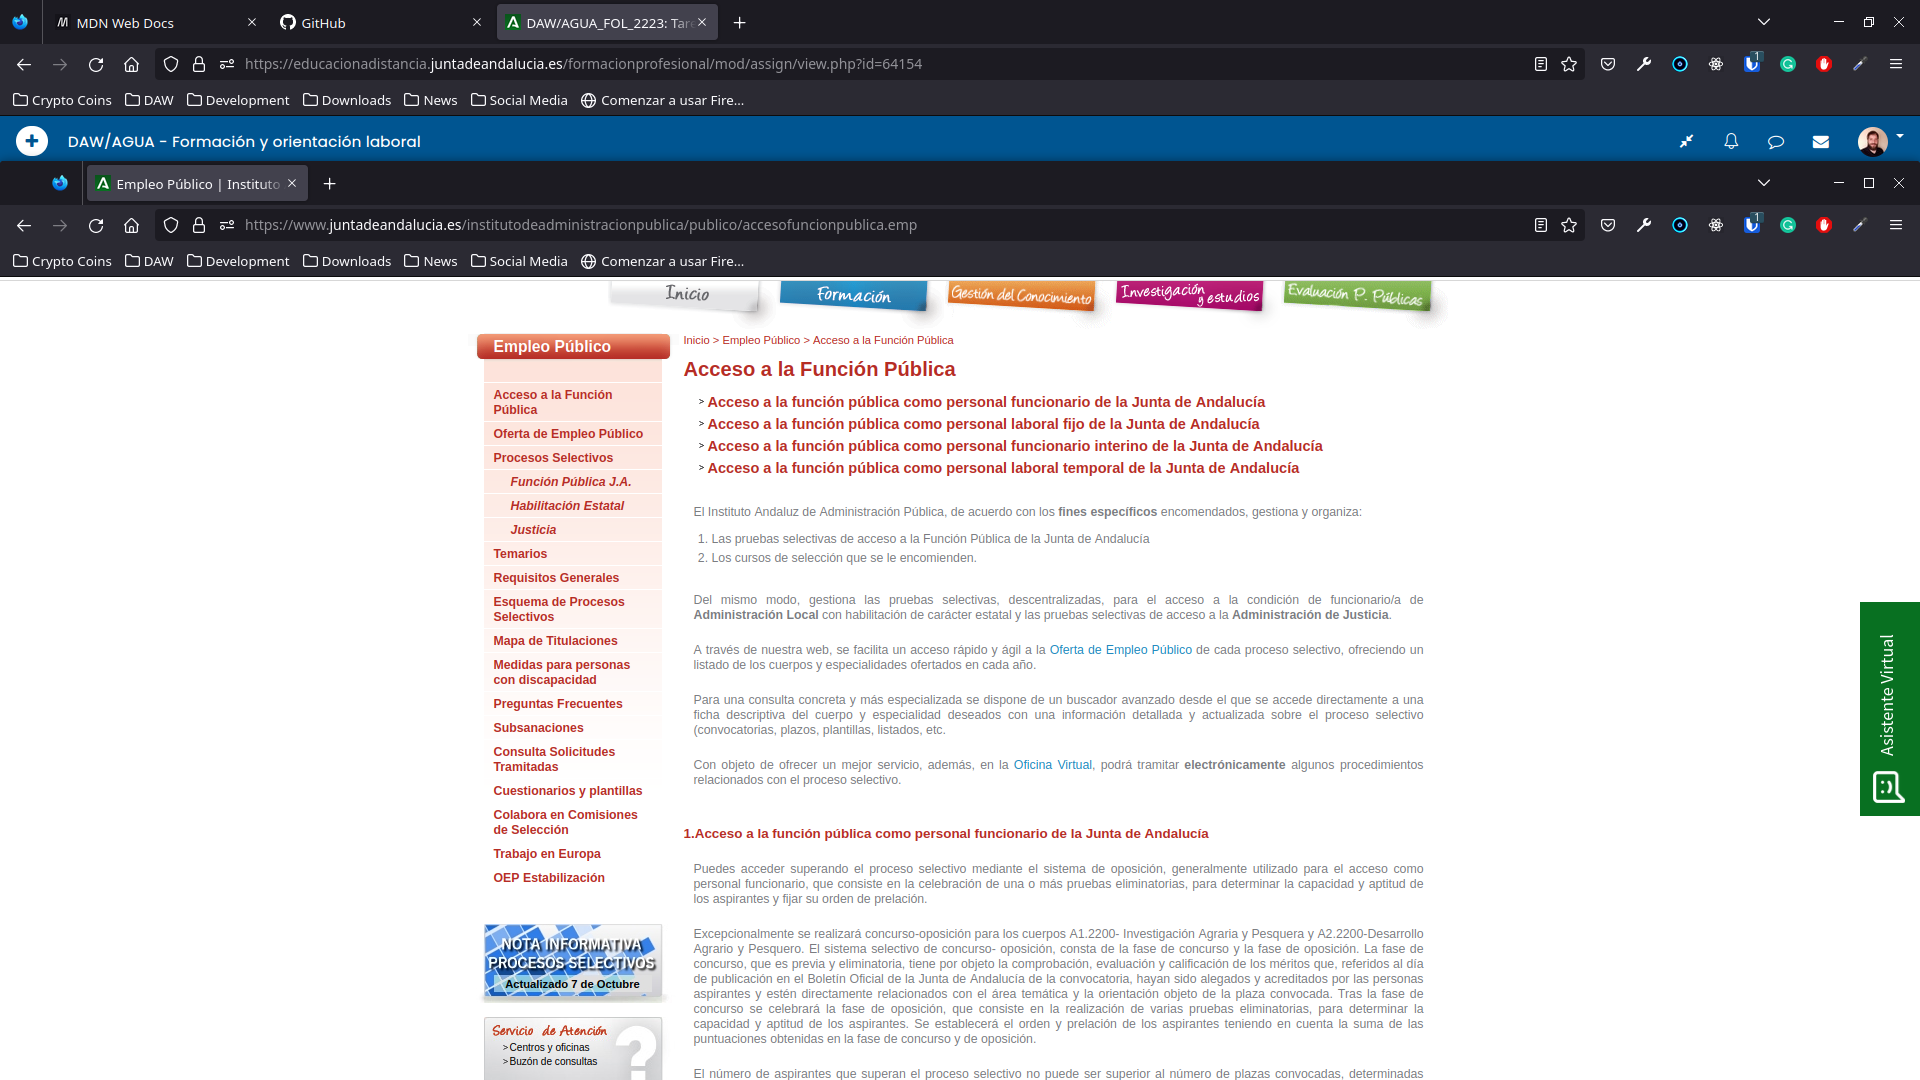
\includegraphics[scale=0.25]{empleo-iaap.png}
        \caption{Sección de Empleo Público del IAAP}
    \end{figure}
\end{enumerate}

\section{Actividad 4}
\subsection{Enunciado}

\begin{enumerate}[label={(\alph*)}]
    \item Realiza una valoración personal reflexionando sobre la importancia de la formación permanente en el sector de la informática y medios a través de los que puedes hacerlo.
    \item Busca una página web/enlace donde aparezca información relacionada con el sector de los estudios que estás cursando ( salidas profesionales, condiciones laborales, oposiciones convocadas,  foros del sector, ofertas de empleo….) Deberás colgarla en el foro y  comentarla. Debes realizar una captura de esta aportación al foro y añadirla a la tarea. La información que subas al foro no podrá haber sido expuesta por otro compañer@ y una sola aportación para que sea igualmente asequible para tod@s.
\end{enumerate}

\subsection{Solución}

\begin{enumerate}[label={(\alph*)}]
    \item En el sector de la informática en general, y más concretamente en el desarrollo de software, la formación continua es imprescindible. Esto se debe a que es un sector muy dinámico donde continuamente están apareciendo nuevas tecnologías, herramientas, paradigmas, etc... Así, es vital para mantener el puesto de trabajo u optar a mejores posiciones la formación continua y la actualización de los conocimientos.

    Los medios de los que nos podemos ayudar para esta formación continua son muy variados. A continuación se muestra una lista con diferentes medios:
    \begin{itemize}
        \item \textbf{Cursos de Formación de la Administración Pública}: tenemos una variedad de cursos de formación y especialización ofertados por las diferentes administraciones públicas. Aquí podemos incluir, por ejemplo, los Cursos de Formación para el Empleo, Formación Ocupacional, Cursos de Especialización, etc... El problema con estos cursos es que el sector del desarrollo de software evoluciona con demasiada rapidez, y los contenidos suelen quedarse desactualizados rápidamente.

        \item \textbf{Plataformas Online de Formación}
    \end{itemize}
    \item
\end{enumerate}









% Bibliography

\newpage
\bibliography{citas}
\bibliographystyle{unsrt}

\end{document}